\documentclass[tikz]{standalone}


\usepackage{xcolor}
\usepackage[inline,shortlabels]{enumitem}

\usepackage{tikz}
\usetikzlibrary{chains, shapes, calc, fit}

\newcommand{\red}[1]{{\color{red} #1}}
\def\todo{\red{TODO}}

\begin{document}

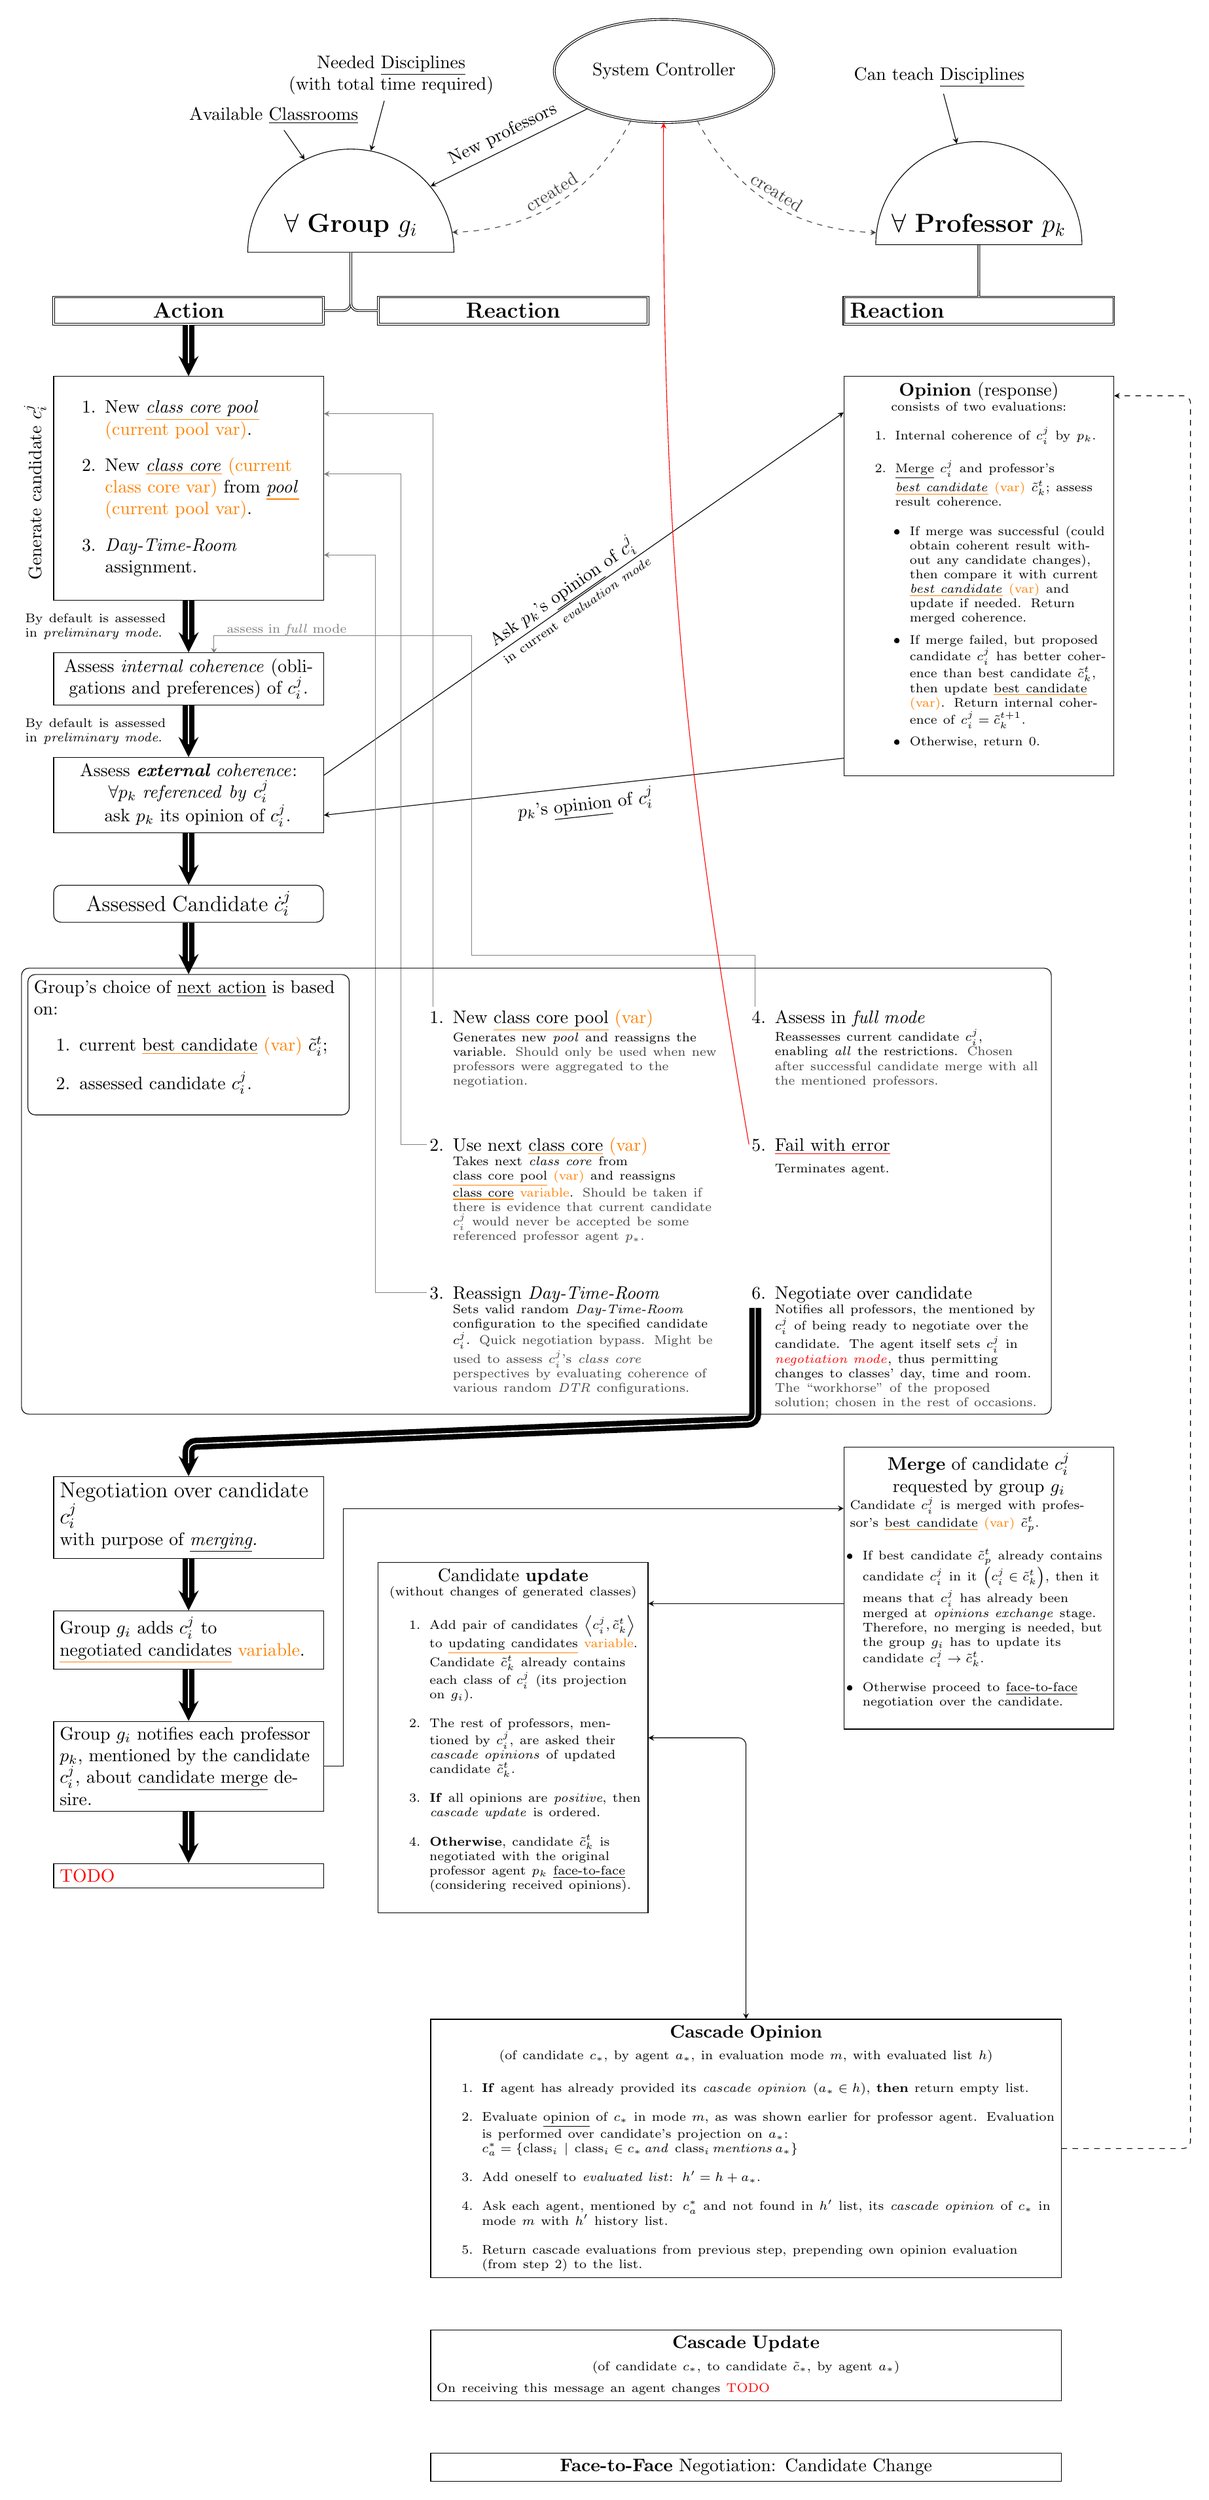
\begin{tikzpicture}[
  start chain=0 going below,
  gact/.style={on chain=0, text width=5cm},
  start chain=1 going below,
  gmsg/.style={on chain=1, text width=5cm},
  start chain=2 going below,
  bothmsg/.style={on chain=2, text width=12cm},
  start chain=3 going below,
  pmsg/.style={on chain=3, text width=5cm},
  flow/.style={draw, ->, >=stealth, double, line width=3pt},
  msg/.style={draw, ->, >=stealth, sloped},
  center/.style={align=center},
  ]

% from http://tex.stackexchange.com/questions/102250/how-to-position-one-node-relative-to-another-node-at-a-certain-angle-in-tikz-tak#
\tikzset{
    position/.style args={#1:#2 from #3}{
        at=(#3.#1), anchor=#1+180, shift=(#1:#2)
    }
}

% from http://tex.stackexchange.com/questions/71478/how-to-center-one-node-exactly-between-two-others-with-tikz
\tikzset{
    between/.style args={#1 and #2}{
         at = ($(#1)!0.5!(#2)$)
    }
}

\newcommand{\var}[2]{%
  \colorlet{temp}{.}\color{orange}\underline{\color{temp}#1} (#2var)\color{temp}%
}

\newcommand{\variable}[1]{%
  \colorlet{temp}{.}\color{orange}\underline{\color{temp}#1} variable\color{temp}%
}

\newcommand{\darkgray}[1]{{\color{darkgray} #1}}

%% I. Creation
\begin{scope}
  %%% Controller
  \node[draw, ellipse, double, minimum width=4cm, minimum height=2cm]
    (Controller) { System Controller };

  %%% Group
  \node[draw, semicircle, minimum width=4cm, minimum height=2cm,
        left=2cm of Controller, yshift=-3cm
        ]
    (Gs) {\Large $\forall$ \textbf{Group} $g_i$ };

  \node[position=75:1cm from Gs,
        text width=5cm, align=center] (DsG)
    {Needed \underline{Disciplines} \\ (with total time required)};
  \node[position=125:0.7cm from Gs,
        text width=5cm, align=center] (Rs)
    {Available \underline{Classrooms}};

  \draw[->, msg, dashed, darkgray]
    (Controller) edge [bend left]
                 node[above] {\darkgray{created}}
    (Gs);

  \draw[->, msg]
    (Controller) -- node[above] {New professors}
    (Gs);


  \draw[->, msg] (DsG) -- (Gs);
  \draw[->, msg] (Rs)  -- (Gs);

  %%% Group Act Thread
  \node[below=of Gs ] (G-between) {};
  \node[gact, center, draw, double,
        left=0.4cm of G-between
        ]
    (G-act) {\large \textbf{Action} };

  %%% Group Message Thread
  \node[gmsg, center, draw, double,
        right=0.4cm of G-between
        ]
    (G-msg) {\large \textbf{Reaction}};

  \draw[double, rounded corners] (Gs) |- (G-act);
  \draw[double, rounded corners] (Gs) |- (G-msg);


  %%% Professor
  \node[draw, semicircle, minimum width=4cm, minimum height=2cm,
        right=2cm of Controller, yshift=-3cm
        ]
    (Ps) {\Large $\forall$ \textbf{Professor} $p_k$ };

  \node[position=105:1cm from Ps,
        text width=5cm, align=center] (DsP)
    {Can teach \underline{Disciplines}};

  \draw[->, msg, dashed, darkgray]
    (Controller) edge[bend right]
                 node[above] {\darkgray{created}}
    (Ps);

  \draw[->, msg] (DsP) -- (Ps);

  %%% Professor Message Thread
  \node[pmsg, draw, double,
        below=of Ps]
    (P-msg) {\large \textbf{Reaction} };

  \draw[double] (Ps) -- (P-msg);


  %%% Both Message Handling
  \node[bothmsg, between=G-msg and P-msg] (msg-both) {};

\end{scope}



%% II. Start - Group
\begin{scope}

  \node[gact, draw,
        label={[rotate=90, xshift=50pt, yshift=10pt]left:{Generate candidate $c_i^j$}}
        ] (G-c-create) {
      \vbox{
      \begin{enumerate}
        \item New \var{\emph{class core pool}}{current pool }.
        \item New \var{\emph{class core}}{current class core }\
              from \var{\emph{pool}}{current pool }.
        \item \emph{Day-Time-Room} assignment.
      \end{enumerate}}
    };

  \node[gact, center, draw] (G-c-internal) {
    Assess \emph{internal coherence} (obligations and preferences) of $c_i^j$.};

  \node[gact, center, draw] (G-c-external) {
    Assess \emph{\textbf{external} coherence}: \\
    $\forall p_k \mathit{~referenced~by~} c_i^j$
      \\\quad ask $p_k$ its opinion of $c_i^j$.
    };

  \node[gact, center, draw, rounded corners] (G-c-assessed)
    {\large Assessed Candidate $\dot{c}_i^j$};

  \draw[flow] (G-act) -- (G-c-create);
  \draw[flow] (G-c-create)
              -- node [text width=3cm, left]
                    {\scriptsize By default is assessed in \emph{preliminary mode}.\\}
              (G-c-internal);
  \draw[flow] (G-c-internal)
              -- node [text width=3cm, left]
                    {\scriptsize By default is assessed in \emph{preliminary mode}.\\}
              (G-c-external);
  \draw[flow] (G-c-external) -- (G-c-assessed);

\end{scope}

%% Professor: Opinion.
\begin{scope}
  \node[pmsg, center, draw] (P-opinion) {
    \textbf{Opinion} (response)
    {\scriptsize consists of two evaluations:
    \begin{enumerate}
      \item Internal coherence of $c_i^j$ by $p_k$.
      \item \underline{Merge} $c_i^j$ and professor's
            \var{\emph{best candidate}}{}\ $\tilde{c}_k^t$;
            assess result coherence.
            \begin{itemize}[leftmargin=8pt]
              \item If merge was successful (could obtain coherent result without
                    any candidate changes), then compare it with current
                    \var{\emph{best candidate}}{}\ and update if needed.
                    Return merged coherence.
              \item If merge failed, but proposed candidate $c_i^j$ has better
                    coherence than best candidate $\tilde{c}_k^t$,
                    then update \var{best candidate}{}.
                    Return internal coherence of $c_i^j = \tilde{c}_k^{t+1}$.
              \item Otherwise, return 0.
            \end{itemize}
    \end{enumerate}
    }};
\end{scope}

%% Opinions exchange.
\begin{scope}
  \draw[msg] ($(G-c-external.north east) - (0,10pt)$)
             -- node[midway, text width=4cm, yshift=3pt]
               {Ask $p_k$'s \underline{opinion} of $c_i^j$ \\
                {\scriptsize in current \emph{evaluation mode}}
               }
             ($(P-opinion.north west) - (0,20pt)$);

  \draw[msg] ($(P-opinion.south west) + (0,10pt)$)
             -- node[below] {$p_k$'s \underline{opinion} of $c_i^j$ }
             ($(G-c-external.south east) + (0,10pt)$);
\end{scope}


%% III. Decision
\begin{scope}
  \node[gact, text width=6cm, draw, rounded corners]
    (Decide)
    {
      Group's choice of \underline{next action} is based on:
      \begin{enumerate}
        \item current \var{best candidate}{}\ $\tilde{c}_i^t$;
        \item assessed candidate $c_i^j$.
      \end{enumerate}
    };

%% Decision 1
  \node[right=of Decide, text width=6cm]
    (Decision-1){
    \begin{enumerate}
    \item New \var{class core pool}{}\\
          {\scriptsize
          Generates new \emph{pool} and reassigns the variable.
          \darkgray{Should only be used when new professors were aggregated
                    to the negotiation.}\\}
     \end{enumerate}
    };

  \draw[msg, gray] (Decision-1.north west) ++(0.62,-0.5)
                -- ++(0,11.5) -- ++(-2.12,0);

%% Decision 2
  \node[below=0 of Decision-1, text width=6cm]
    (Decision-2){
    \begin{enumerate}[start=2]
    \item Use next \var{class core}{}\\
          {\scriptsize
          Takes next \emph{class core} from \var{class core pool}{}\ and reassigns
          \variable{class core}.
          \darkgray{Should be taken if there is evidence that current
                    candidate $c_i^j$ would never be accepted be some referenced
                    professor agent $p_*$.}\\}
     \end{enumerate}
    };

  \draw[msg, gray] (Decision-2.north west) ++(0.5,-0.7)
                -- ++(-0.5,0) -- ++(0,13) -- ++(-1.5,0);

%% Decision 3
  \node[below=0 of Decision-2, text width=6cm]
    (Decision-3){
    \begin{enumerate}[start=3]
    \item Reassign \emph{Day-Time-Room}\\
          {\scriptsize
          Sets valid random \emph{Day-Time-Room} configuration to the specified
          candidate $c_i^j$.
          \darkgray{Quick negotiation bypass.
                    Might be used to assess $c_i^j$'s \emph{class core} perspectives
                    by evaluating coherence of various random \emph{DTR} configurations.}
          \\}
     \end{enumerate}
    };

  \draw[msg, gray] (Decision-3.north west) ++(0.5,-0.7)
                -- ++(-1,0) -- ++(0,14.3) -- ++(-1,0);

%% Decision 4
  \node[anchor=north west, at={([xshift=0cm]Decision-1.north east)},
        text width=6cm]
    (Decision-4) {
    \begin{enumerate}[start=4]
    \item Assess in \emph{full mode}\\
          {\scriptsize
          Reassesses current candidate $c_i^j$, enabling \emph{all} the restrictions.
          \darkgray{Chosen after successful candidate merge with all the mentioned
                    professors.}\\}
     \end{enumerate}
    };

  \draw[msg, gray] (Decision-4.north west) ++(0.62,-0.5)
                -- ++(0,1) -- ++(-5.5,0)
                -- ++(0,6.2) -- ++(-5,0)
                -- node[label={[yshift=8pt]above:{\scriptsize
                        assess in \emph{full} mode}}
                    ]{} ++(0,-0.35);

%% Decision 5
  \node[anchor=north west, at={([xshift=0cm]Decision-2.north east)},
        text width=6cm]
    (Decision-5) {
    \begin{enumerate}[start=5]
    \item \colorlet{temp}{.}
          \red{\underline{\color{temp}Fail with error}}\\
          {\scriptsize Terminates agent. }
     \end{enumerate}
    };

  \draw[red] (Decision-5.north west) ++(0.5,-0.7)
                % -- ++(-0.5,0)
                edge [msg, bend left=5pt]
                (Controller);

%% Decision 6
  \node[anchor=north west, at={([xshift=0cm]Decision-3.north east)},
        text width=6cm]
    (Decision-6) {
    \begin{enumerate}[start=6]
    \item Negotiate over candidate\\
          {\scriptsize
          Notifies all professors, the mentioned by $c_i^j$ of being ready
          to negotiate over the candidate. The agent itself sets $c_i^j$ in
          \red{\emph{negotiation mode}}, thus permitting changes to classes' day, time and room.
          \darkgray{The ``workhorse'' of the proposed solution; chosen in the
          rest of occasions.}\\}
     \end{enumerate}
    };

%% Decisions flow
  \draw[flow] (G-c-assessed) -- (Decide);

  \node[draw, rounded corners, fit=(Decide) (Decision-4) (Decision-6)]{};

\end{scope}


%% IV. Candidate Merge Negotiation
\begin{scope}
  \node[gact, draw, yshift=-6cm]
    (G-negotiate)
    {{\large Negotiation over candidate $c_i^j$} \\
     with purpose of \emph{\underline{merging}.}};

  \node[gact, draw]
    (G-neg-prepare)
    {Group $g_i$ adds $c_i^j$ to \variable{negotiated candidates}.};

  \node[gact, draw]
    (G-neg-notify)
    {Group $g_i$ notifies each professor $p_k$, mentioned by the candidate $c_i^j$,
     about \underline{candidate merge} desire.};

  \node[gact, draw] (G-neg-todo) {\todo};

%% Flow
  \node[above=0.5cm of G-negotiate] (G-negotiate-above){};

  \draw[flow, rounded corners]
    (Decision-6.north west) ++ (0.62,-1)
    -- ++(0,-2.2) -- ($(G-negotiate-above)$) -- (G-negotiate);

  \draw[flow] (G-negotiate) -- (G-neg-prepare);
  \draw[flow] (G-neg-prepare) -- (G-neg-notify);
  \draw[flow] (G-neg-notify) -- (G-neg-todo);
\end{scope}

%% Professor: Merge. %  - Beginning
\begin{scope}
  \node[pmsg, yshift=-12cm, draw]
    (P-merge)
    {{\centering \textbf{Merge} of candidate $c_i^j$ requested by group $g_i$\\}
    {\scriptsize
     Candidate $c_i^j$ is merged with professor's \var{best candidate}{}\
     $\tilde{c}_p^t$.
     \begin{itemize}[leftmargin=7pt]
       \item If best candidate $\tilde{c}_p^t$ already contains candidate $c_i^j$
             in it $\left( c_i^j \in \tilde{c}_k^t \right)$, then it means that
             $c_i^j$ has already been merged at \emph{opinions exchange} stage.
             Therefore, no merging is needed, but the group $g_i$ has to update
             its candidate $c_i^j \rightarrow \tilde{c}_k^t$.
       \item Otherwise proceed to \underline{face-to-face} negotiation over
             the candidate.
     \end{itemize}
    }};
\end{scope}

%% Group: Merge -- Candidate Update
\begin{scope}
  \node[gmsg, center, yshift=-23cm, draw]
    (G-merge-update)
    {Candidate \textbf{update}\\
    {\scriptsize (without changes of generated classes)
     \begin{enumerate}
       \item Add pair of candidates $\left< c_i^j, \tilde{c}_k^t \right>$ to
             \variable{updating candidates}.
             Candidate $\tilde{c}_k^t$ already contains each class of $c_i^j$
             (its projection on $g_i$).
       \item The rest of professors, mentioned by $c_i^j$, are asked their
             \emph{cascade opinions} of updated candidate $\tilde{c}_k^t$.
       \item \textbf{If} all opinions are \emph{positive}, then \emph{cascade update}
             is ordered.
       \item \textbf{Otherwise}, candidate $\tilde{c}_k^t$ is negotiated with
             the original professor agent $p_k$ \underline{face-to-face}
             (considering received opinions).
     \end{enumerate}
    }};

  %% Merge messages
  \draw[msg] (G-neg-notify) -- ++(3,0) -- ++(0,5) node (tmp) {} -- (P-merge.west |- tmp);
  \draw[msg] let \p{P}=($(P-merge.west) - (0,0.3cm)$)
             in (\p{P}) -- (G-merge-update.east |- \p{P});

\end{scope}


%% Cascade Opinion
\begin{scope}
  \node[bothmsg, yshift=-32cm, draw]
    (Cascade-Opinion)
    {{\centering \textbf{Cascade Opinion} \\
                 {\scriptsize (of candidate $c_*$,
                               by agent $a_*$,
                               in evaluation mode $m$,
                               with evaluated list $h$)} \\}
     {\scriptsize
      \begin{enumerate}
        \item \textbf{If} agent has already provided its \emph{cascade opinion}
              $\left( a_* \in h \right)$, \textbf{then} return empty list.
        \item Evaluate \underline{opinion} of $c_*$ in mode $m$,
              as was shown earlier for professor agent.
              Evaluation is performed over candidate's projection on $a_*$:
              $c_a^* = \{\mathrm{class}_i ~|~
                            \mathrm{class}_i \in c_* \,\mathit{and}\
                            \mathrm{class}_i \,\mathit{mentions}\, a_*\}$
        \item Add oneself to \emph{evaluated list}: $h' = h + a_*$.
        \item Ask each agent, mentioned by $c_a^*$ and not found in $h'$ list,
              its \emph{cascade opinion} of $c_*$ in mode $m$
              with $h'$ history list.
        \item Return cascade evaluations from previous step,
              prepending own opinion evaluation (from step 2) to the list.
      \end{enumerate}
     }};

  %% Cascade Opinion Messages
  \draw[msg, <->, rounded corners] (G-merge-update) -| (Cascade-Opinion);
  \draw[msg, ->, dashed, rounded corners]
    (Cascade-Opinion.east) -- ++(2.5,0) |- ($(P-opinion.east) + (0,3.5cm)$);
\end{scope}

%% Cascade Update
\begin{scope}
  \node[bothmsg, draw] (Cascade-Update)
    {{\centering \textbf{Cascade Update} \\
                 {\scriptsize (of candidate $c_*$,
                               to candidate $\tilde{c}_*$,
                               by agent $a_*$)} \\}
    {\scriptsize
     On receiving this message an agent changes \todo
    }\\};
\end{scope}

%% V. Candidate Change Negotiation
\begin{scope}
  \node[bothmsg, draw]
    (face-2-face)
    {{\centering \textbf{Face-to-Face} Negotiation: Candidate Change \\}

    };
\end{scope}

\end{tikzpicture}

\end{document}
